\subsection{RQ1. Comparative Study on C\# Dataset}
\label{rq1:sec}

\begin{table}[t]
	\caption{RQ1. Comparison on C\# Dataset ($Accuracy^c$\%)}
	\vspace{-0.1in}
	\begin{center}
		\footnotesize
		\tabcolsep 4pt
		\renewcommand{\arraystretch}{1} \begin{tabular}{p{0.2cm}<{\centering}|p{0.25cm}<{\centering}p{0.25cm}<{\centering}p{0.25cm}<{\centering}|p{0.25cm}<{\centering}p{0.25cm}<{\centering}p{0.25cm}<{\centering}|p{0.25cm}<{\centering}p{0.25cm}<{\centering}p{0.25cm}<{\centering}|p{0.25cm}<{\centering}p{0.25cm}<{\centering}p{0.25cm}<{\centering}|p{0.25cm}<{\centering}p{0.25cm}<{\centering}p{0.25cm}<{\centering}}
			
			\hline
		\multirow{2}{*}{}          & \multicolumn{3}{c|}{Barnett {\em et al.}} & \multicolumn{3}{c|}{Herzig {\em et al.}} & \multicolumn{3}{c|}{$\delta-$PDG + CV} & \multicolumn{3}{c|}{Flexeme} & \multicolumn{3}{c}{\bf {\tool}}\\
		\cline{2-16}
		 & 2 & 3 & OA & 2 & 3 & OA & 2 & 3 & OA & 2 & 3 & OA & 2 & 3 & OA \\
			\hline
			CL   & 14 & *    & 14 & 28 & *    & 28 & 34 & *    & 34 & 34 & *    & 34 & 46 & *    & 46 \\
			CM   & *    & *    & *    & *    & *    & *    & *    & *    & *    & *    & *    & *    & *    & *    & *    \\
			HF   & 10 & 13 & 11 & 27 & 29 & 28 & 34 & 37 & 35 & 30 & 35 & 31 & 43 & 48 & 45 \\
			HU   & 13 & *    & 13 & 27 & *    & 27 & 30 & *    & 30 & 33 & *    & 33 & 44 & *    & 44 \\
			LE   & 8 & 6 & 8 & 29 & 24 & 29 & 35 & 34 & 35 & 33 & 36 & 33 & 44 & 47 & 45\\
			NA   & *    & *    & *    & *    & *    & *    & *    & *    & *    & *    & *    & *    & *    & *    & *    \\
			NJ   & 7 & *    & 7 & 28 & *    & 28 & 34 & *    & 34 & 27 & *    & 27 & 41 & *    & 41 \\
			NI   & 10 & *    & 10 & 26 & *    & 26 & 37 & *    & 37 & 32 & *    & 32 & 46 & *    & 46 \\
			RS   & 9 & 11 & 9 & 31 & 30 & 31 & 30 & 36 & 31 & 32 & 35 & 33 & 42 & 49 & 43\\
			\hline
			OA   & 8 & 6 & 8 & 31 & 25 & 29 & 35 & 34 & 35 & 32 & 36 & 33 & {\bf 44} & {\bf 47} & {\bf 45} \\
			\hline
		\end{tabular}
		\label{RQ1-result-1}
		CL:Commandline, CM:CommonMark, HF:Hangfire, HU:Humanizer, LE:Lean, NA:Nan cy, NJ:Newtonsoft.Json, NI:Ninject, RS:RestSharp, OA: Overall, *: No avail data point.
	\end{center}
\end{table}

\begin{table}[t]
	\caption{RQ1. Comparison on C\# Dataset ($Accuracy^a$\%)}
	\vspace{-0.1in}
	\begin{center}
		\footnotesize
		\tabcolsep 4pt
		\renewcommand{\arraystretch}{1} \begin{tabular}{p{0.2cm}<{\centering}|p{0.25cm}<{\centering}p{0.25cm}<{\centering}p{0.25cm}<{\centering}|p{0.25cm}<{\centering}p{0.25cm}<{\centering}p{0.25cm}<{\centering}|p{0.25cm}<{\centering}p{0.25cm}<{\centering}p{0.25cm}<{\centering}|p{0.25cm}<{\centering}p{0.25cm}<{\centering}p{0.25cm}<{\centering}|p{0.25cm}<{\centering}p{0.25cm}<{\centering}p{0.25cm}<{\centering}}
			
			\hline
			\multirow{2}{*}{}          & \multicolumn{3}{c|}{Barnett {\em et al.}} & \multicolumn{3}{c|}{Herzig {\em et al.}} & \multicolumn{3}{c|}{$\delta-$PDG + CV} & \multicolumn{3}{c|}{Flexeme} & \multicolumn{3}{c}{\bf {\tool}}\\
			\cline{2-16}
			& 2 & 3 & OA & 2 & 3 & OA & 2 & 3 & OA & 2 & 3 & OA & 2 & 3 & OA \\
			\hline
			CL   & 13 & *    & 13 & 68 & *    & 68 & 80 & *    & 80 & 85 & *    & 85 & 90 & *    & 90 \\
			CM   & *    & *    & *    & *    & *    & *    & *    & *    & *    & *    & *    & *    & *    & *    & *    \\
			HF   & 06 & 11 & 07 & 71 & 59 & 68 & 81 & 86 & 82 & 80 & 89 & 82 & 84 & 91 & 86 \\
			HU   & 14 & *    & 14 & 66 & *    & 66 & 79 & *    & 79 & 83 & *    & 83 & 89 & *    & 89 \\
			LE   & 13 & 10 & 12 & 72 & 64 & 70 & 80 & 83 & 81 & 84 & 86 & 84 & 87 & 90 & 88\\
			NA   & *    & *    & *    & *    & *    & *    & *    & *    & *    & *    & *    & *    & *    & *    & *    \\
			NJ   & 10 & *    & 10 & 68 & *    & 68 & 85 & *    & 85 & 75 & *    & 75 & 83 & *    & 83 \\
			NI   & 15 & *    & 15 & 64 & *    & 64 & 83 & *    & 83 & 81 & *    & 81 & 91 & *    & 91 \\
			RS   & 12 & 17 & 13 & 76 & 78 & 76 & 74 & 81 & 76 & 82 & 87 & 83 & 87 & 88 & 87\\
			\hline
			OA   & 13 & 10 & 12 & 72 & 64 & 70 & 79 & 83 & 81 & 82 & 86 & 83 & {\bf 88} & {\bf 91} & {\bf 89} \\
			\hline
		\end{tabular}
		\label{RQ1-result-2}
		CL:Commandline, CM:CommonMark, HF:Hangfire, HU:Humanizer, LE:Lean, NA:Nan cy, NJ:Newtonsoft.Json, NI:Ninject, RS:RestSharp, OA: Overall, *: No avail data point.
	\end{center}
\end{table}


%\textcolor{red}{Yi: consider adding Table 2 in Flexeme paper to our paper on the statistics of the data}.

%\textcolor{red}{Yi: add Figure 4(a) in Flexeme paper to our paper to show the accuracy distribution for different numbers of concerns.}

Table~\ref{RQ1-result-1} shows the comparison on $Accuracy^{c}$ when
accuracy was measured on the changed statements. As seen, {\tool}
improves Barnett {\em et al.}, Herzig {\em et al.}, $\sigma-$PDG+CV,
and Flexeme in overall $Accuracy^c$ by {\bf 462.5\%, 55.2\%, 28.6\%},
and {\bf 36.4\%}, respectively. As seen in Table~\ref{RQ1-result-2},
when $Accuracy^{a}$ is measured on all the statements (changed and
un-changed) in a commit, the results for all models are higher because
they have correct classifications for the changed statements by
default. We include $Accuracy^{a}$ for the comparison purpose with
Flexeme (as its authors used this metric in their paper). As seen,
{\tool} also improves Barnett {\em et al.}, Herzig {\em et al.},
$\sigma-$PDG+CV, and Flexeme by {\bf 641.7\%, 27.1\%, 9.9\%,} and {\bf
  7.3\%} in overall $Accuracy^{a}$, respectively. Moreover, {\tool}'s
accuracies are consistently better than those of the baselines for all
the subject projects with different numbers of concerns in the
commits.

{\color{red}{why some data points are not available?}}

%Table~\ref{RQ1-result-1} and Table~\ref{RQ1-result-2} show the results about comparing \tool with baselines on C\# dataset. Table~\ref{RQ1-result-1} shows the $Accuracy^c$ results that \tool can improve the $Accuracy^c$ by $462.5\%, 55.2\%, 28.6\%, $ and $36.4\%$ compared with Barnett et al., Herzig et al., $\sigma-$PDG + CV, and Flexeme, respectively. Table~\ref{RQ1-result-2} shows the $Accuracy^a$ results that \tool can improve the  $Accuracy^a$ by $641.7\%, 27.1\%, 9.9\%, $ and $7.3\%$ comparing with Barnett et al., Herzig et al., $\sigma-$PDG + CV, and Flexeme, respectively. On all projects, \tool have the best overall performance compared with baselines, which proves the high accuracy of \tool on untangling task on C\# dataset.


\begin{figure}
	\centering
	\begin{subfigure}{0.235\textwidth}
		\centering
		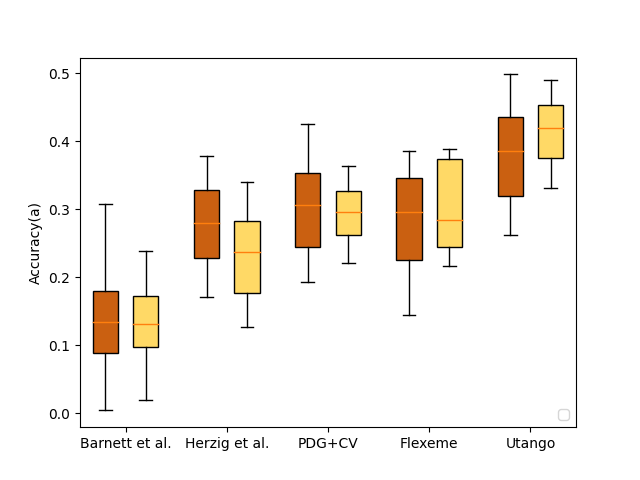
\includegraphics[width=1.7in]{figures/RQ_1_1.png}
                \vspace{-16pt}
		\caption{$Accuracy^c$}
		\label{RQ1-result-3-1}
	\end{subfigure}
	\begin{subfigure}{0.235\textwidth}
		\centering
		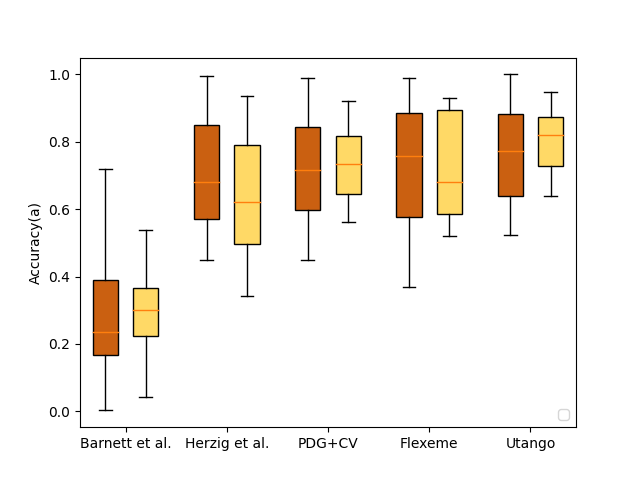
\includegraphics[width=1.7in]{figures/RQ_1_2.png}
                \vspace{-16pt}
		\caption{$Accuracy^a$}
		\label{RQ1-result-3-2}
	\end{subfigure}
        \vspace{-12pt}
	\caption{Boxplots for the Results in Table~\ref{RQ1-result-1} and Table~\ref{RQ1-result-2}. Orange Boxes: 2 concerns data, Yellow Boxes: 3 concerns data}
	\label{RQ1-result-3}
\end{figure}

Figure~\ref{RQ1-result-3} shows the boxplots for both $Accuracy^c$ and
$Accuracy^a$ results in Tables~\ref{RQ1-result-1}
and~\ref{RQ1-result-2}. The orange boxes are for the commits with two
concerns, while the yellow ones are for those with three concerns. As
seen, the median accuracy of {\tool} is higher than those of all
baselines on both types of two and three concerns. Moreover, the gap
between {\tool} and the baselines in $Accuracy^{c}$ is larger than the
gap between them in $Accuracy^{a}$ because all models have correct
classifications by default for the changed statements, which are many
more than the changed ones.

%By considering the average accuracy reported in Table~\ref{RQ1-result-1} and Table~\ref{RQ1-result-2}, \tool has been proved to have the best results on the C\# dataset when compared with all baselines.

%\vspace{3pt}
\noindent {\bf Further Analysis.} For further comparison, we report
that there are {\bf 92} commits that {\tool} correctly classified
100\% of all the changed statements, while there are {\bf 64} commits
that the best baseline, Flexeme, correctly classified all the
changed statements. Both models correctly classified 100\% all the
changed statements of {\bf 13} commits.  Those commits contain from
2--9 changed statements.
       


%do an extra analysis on the number of tangled commits that \tool or the best-performed baseline $Flexeme$ can $100\%$ cluster each changed statement correctly. The results show that there are $92$ commits that \tool can $100\%$ cluster the changed statements correctly while there are $64$ commits that $Flexeme$ can $100\%$ cluster the changed statements correctly. The overlapping between them is about $13$ commits. And the concerns in these commits often have $2-9$ statements inside. The number of commits that \tool can $100\%$ correctly cluster changed statements is limited because there are many concerns in the commits containing many changed statements. It is very hard for \tool to cluster each of them correctly at the same time perfectly. That's also why the concerns in $100\%$ correctly clustered commits often have the limited size from $1$ statements to $9$ statements.

\begin{figure}[t]
	\centering 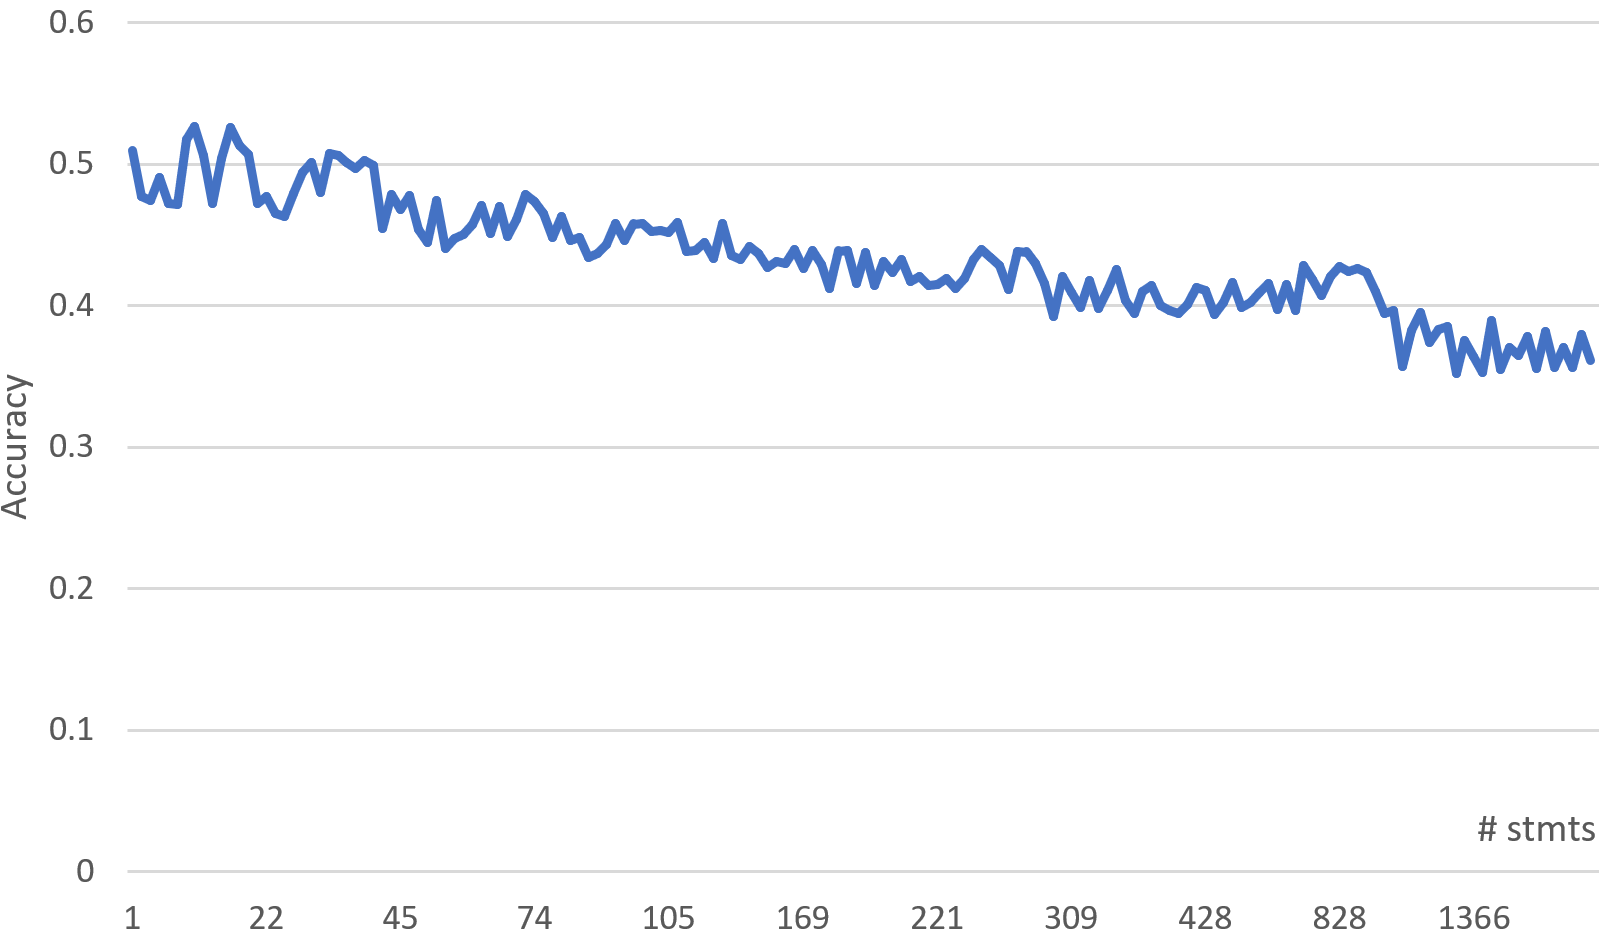
\includegraphics[width=1.8in]{figures/accuracy-concerns.png}
	\vspace{-6pt}
	\caption{Accuracy for Concerns with Diff. Numbers of Stmts}
	\label{acc-concerns}
\end{figure}

To better understand {\tool}'s performance on different sizes of
concerns, we collected all concerns with different numbers of changed
statements and measured the corresponding accuracies for them.  As
seen in Figure~\ref{acc-concerns}, $Accuracy^{c}$ values for the concerns of
small sizes (having 1--22 changed statements) are higher (ranging
from 47\%--54\%). That is, among all the changed statements, {\tool}
correctly classified about 50\% of them into the correct clusters.
For the larger concerns, $Accuracy^{c}$ decreases as expected because
it is more challenging to get correct classifications for more changed
statements in a concern. However, $Accuracy^{c}$ decreases gradually with the
lowest value of around 36\%. Note that there are some commits with the
addition of large files with $>$1.3k lines.

%To better understand the performance of \tool on different sizes of concerns, we collect all concerns, and their size is from $1$ statements to $189$ statements. Then, by dividing them into four groups with the same amount of concerns following the order of the size, \tool can achieve $0.49$, $0.47$, $0.44$, and $0.40$ $Accuracy^c$ on group 1 (with the smallest size of concerns) to group 4 (with the biggest size of concerns), respectively. The results show that \tool can perform slightly better on the smaller size of concerns, but the gap on the results is not too big and still in the acceptable range.
